\documentclass[11pt]{article}

% EMNLP 2026 Demo Track is single-blind: authors are named.
% [preprint] = non-anonymous + page numbers (no line numbers).
% Switch to [final] for the camera-ready.
\usepackage[preprint]{acl}

% Standard package includes
\usepackage{times}
\usepackage{latexsym}

% For proper rendering and hyphenation of words containing Latin characters.
\usepackage[T1]{fontenc}
\usepackage[utf8]{inputenc}
\usepackage{microtype}
\usepackage{inconsolata}

% Figures and diagrams.
\usepackage{graphicx}
\usepackage{tikz}
\usetikzlibrary{positioning, arrows.meta, calc}

% Tables and math.
\usepackage{booktabs}
\usepackage{amsmath}
\usepackage{amssymb}

% Inline author note for proposed design choices that need confirmation.
% xcolor is already loaded by acl.sty.
\newcommand{\designnote}[1]{\textcolor{red}{\textit{[TODO: #1]}}}

\title{Humanly: Process Evidence for Human-AI Writing}

% EMNLP 2026 Demo Track is single-blind: fill in real names and affiliations.
\author{First Author \\
  Affiliation / Address line 1 \\
  \texttt{email@domain} \\\And
  Second Author \\
  Affiliation / Address line 1 \\
  \texttt{email@domain} \\}

\begin{document}
\maketitle

\begin{abstract}
Large language models make it increasingly difficult to infer how a piece of writing was produced from the final text alone. This is a policy problem, not only a detection problem: in classrooms, peer review, and personal certification, AI assistance may be allowed, limited, or prohibited depending on the task. We present \textsc{Humanly}, a provenance-first writing platform that records how a draft comes together and turns that record into verifiable process evidence. Writers draft in a tracked editor; task owners configure AI access, paste rules, character limits, and time limits; and the system records typing, paste, focus, selection, and AI-assist events. At completion, \textsc{Humanly} issues a certificate and verification link that connect the final text to typed/pasted statistics, AI-use logs, and replayable writing history. We evaluate \textsc{Humanly} from two angles: first, by comparing final-text AI detectors and process-replay systems on the policy-compliance questions they can and cannot answer; second, through a human study of whether writers can use \textsc{Humanly} naturally and whether readers can interpret its certificate evidence. The system is deployed at \url{https://app.writehumanly.net/}.
\end{abstract}

\section{Introduction}
\label{sec:intro}

Large language models have changed the status of writing evidence. A fluent final draft no longer tells an instructor whether a student composed the argument, a program chair whether a reviewer engaged with a paper, or a reader whether a writing sample reflects a person's own process. The question is often stated as ``did a human or AI write this?'' Yet in practice the sharper question is policy-compliance: what assistance was allowed for this task, and what evidence shows how the text was produced?

Most existing responses operate after the fact. Text detectors judge whether the final document resembles model output \citep{mitchell2023detectgpt, hans2024binoculars, verma2024ghostbuster}. This can be useful for some fully generated text, but it cannot distinguish many mixed workflows: a human draft polished by AI, a non-native English writer falsely flagged as AI-generated \citep{liang2023gpt}, or an AI draft paraphrased by a humanizer. Process-replay tools improve the situation by showing document history, but replay alone does not necessarily define a task policy, log sanctioned AI use, or issue portable evidence that a writer can share with a reader.

\textsc{Humanly} starts from a different principle: \emph{process beats prediction}. Instead of inferring authorship from style, Humanly records the writing process as it happens. A task owner can configure AI access, paste rules, time limits, and character limits before writing begins. A writer then drafts inside a tracked editor where typed text, paste events, focus changes, selections, and AI interactions are recorded. At the end, Humanly generates a certificate and verification link that connect the final draft to a process record.

This framing allows AI to be treated as a governed part of writing rather than as a binary contaminant. Humanly can be used when AI is disabled, when only AI polishing is allowed, when only chat assistance is allowed, or when full AI assistance is allowed. In each case, the relevant evidence is not whether the final prose ``sounds AI-generated,'' but whether the process matches the rules set for the task.

Our contributions are:
\begin{enumerate}
  \item a deployed, AI-native writing platform that captures write-time provenance and issues verifiable certificates;
  \item configurable writing environments for personal documents and assigned tasks, including four AI-access modes, paste policy, character limits, and time limits;
  \item a comparison and evaluation plan that contrasts Humanly with final-text AI detectors and document-replay tools on policy-compliance questions;
  \item a human-study design for evaluating writer usability, policy clarity, and reader interpretation of certificate evidence.
\end{enumerate}
\designnote{Replace the third and fourth contributions with actual evaluation findings once data collection is complete.}

\section{System Architecture}
\label{sec:architecture}

\textsc{Humanly} is a deployed web platform with three production surfaces: a user portal for writers, an admin dashboard for task owners, and an API/tracker host. The implementation is a TypeScript monorepo: an Express backend with PostgreSQL/TimescaleDB and Redis, a Next.js admin dashboard, a Next.js user portal, a Lexical editor package, a standalone tracker package, and shared validators/types. Figure~\ref{fig:workflow} sketches the current data path.

\begin{figure}[t]
\centering
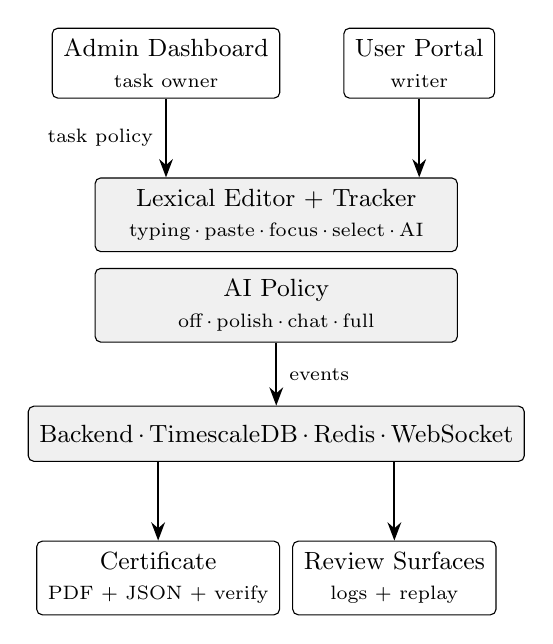
\begin{tikzpicture}[
  every node/.style={font=\small},
  box/.style={draw, rectangle, rounded corners=2pt, align=center, inner sep=4pt, minimum height=7mm},
  core/.style={box, fill=gray!12},
  arr/.style={-Stealth, thick}
]
  \node[box] (admin) {Admin Dashboard\\\scriptsize task owner};
  \node[box, right=8mm of admin] (user) {User Portal\\\scriptsize writer};

  \node[core, below=10mm of admin, xshift=14mm, minimum width=46mm] (editor)
    {Lexical Editor + Tracker\\\scriptsize typing\,$\cdot$\,paste\,$\cdot$\,focus\,$\cdot$\,select\,$\cdot$\,AI};
  \node[core, below=2mm of editor, minimum width=46mm] (ai)
    {AI Policy\\\scriptsize off\,$\cdot$\,polish\,$\cdot$\,chat\,$\cdot$\,full};

  \node[core, below=8mm of ai, minimum width=58mm] (backend)
    {Backend\,$\cdot$\,TimescaleDB\,$\cdot$\,Redis\,$\cdot$\,WebSocket};

  \node[box, below=10mm of backend.south, xshift=-15mm] (cert) {Certificate\\\scriptsize PDF + JSON + verify};
  \node[box, below=10mm of backend.south, xshift=15mm] (review) {Review Surfaces\\\scriptsize logs + replay};

  \draw[arr] (admin.south) -- node[midway, left=1pt] {\scriptsize task policy} (admin.south |- editor.north);
  \draw[arr] (user.south) -- (user.south |- editor.north);
  \draw[arr] (ai.south) -- node[midway, right=1pt] {\scriptsize events} (backend.north);
  \draw[arr] (backend.south -| cert.north) -- (cert.north);
  \draw[arr] (backend.south -| review.north) -- (review.north);
\end{tikzpicture}
\caption{Humanly records the writing process at the editor surface, stores events and document state in the backend, and produces certificate, verification, log, and replay surfaces for later review.}
\label{fig:workflow}
\end{figure}

\paragraph{Writing environments.}
Each document is governed by an environment configuration. The configuration records whether the task is personal or admin-assigned, whether instruction PDFs are present, which AI provider and model are allowed, how much AI use is permitted, whether paste is allowed or blocked, whether start/end windows and a writing timer apply, and whether minimum or maximum character counts are enforced. The current AI-access modes are \textsc{off}, \textsc{polish}, \textsc{chat}, and \textsc{full}. In \textsc{polish}, only selection-level actions such as fixing grammar, improving writing, simplifying, or formalizing are available. In \textsc{chat}, only the agent chat is available. In \textsc{full}, both are available. In \textsc{off}, AI is disabled.

\paragraph{Editor and recording layer.}
Writers draft in a Lexical-based editor instrumented with provenance capture. The system records typing, paste, focus/blur, selection, and AI-assist events as part of the writing session. When AI is enabled, Humanly records both agent-chat interactions and selection-level AI actions, including whether the writer accepts or rejects generated text. This makes AI collaboration part of the process record rather than an invisible side channel.

\paragraph{Task and enrollment layer.}
Admin-assigned tasks are created in the admin dashboard and can be joined through authenticated invite-code enrollment or public share links. A task owner can decide whether a public link allows guest submissions. Public writers must start a Humanly document before submitting; direct public submission is disabled. Signed-in public writers enter the normal task/certificate flow, while guest sessions are mapped to synthetic guest users so the same editor and certificate pipeline can run.

\paragraph{Storage and review layer.}
The backend stores document state, event streams, task enrollments, submissions, AI chat sessions, and AI selection actions. PostgreSQL/TimescaleDB supports high-frequency event storage, while WebSocket channels support live or near-live review surfaces in the admin workflow. \designnote{Verify which live-monitoring surfaces should be shown in the final screenshot set.}

\paragraph{Certificate and verification layer.}
At completion, Humanly generates a certificate containing the document title, generated time, certificate identifier, verification token, typed and pasted character counts, event counts, editing time, and AI-use statistics. Certificates can be exported as JSON and PDF and can be verified through a public URL. When enabled, certificates can include the full text, edit history, replay/log surfaces, and an access-code gate.

\section{Workflows and Use Cases}
\label{sec:workflows}

Humanly supports three primary workflows. Each is organized around the same principle: the relevant artifact is not only the final text, but also the process evidence attached to it.

\subsection{Peer Review of Academic Papers}

Peer review is a natural policy-compliance setting. Venues increasingly need to specify whether reviewers may use LLMs for grammar, polishing, summarization, or substantive review. Final-text detectors cannot tell whether a review reflects a reader's own engagement with the paper or whether an external model produced the main judgment. In Humanly, a program chair can create an assigned review task, attach instruction files or paper context, configure the permitted AI mode, and ask reviewers to write inside the tracked workspace. The resulting certificate gives the chair a process trail: writing duration, typed and pasted content, AI interactions, and replayable history.

\subsection{Classroom Writing Assignments}

Instructors face the same policy problem at a larger scale. Some courses ban AI assistance; others allow grammar correction, brainstorming, or full collaboration. Humanly lets instructors configure those rules before writing starts. Students then write in an environment where the interface itself reflects the permitted mode. On submission, the instructor can review the final text together with typed/pasted statistics, paste-policy evidence, AI-use logs, and certificate metadata. This shifts the interaction from accusation and defense to a shared process record.

\subsection{Personal Writing Certification}

Writers can also use Humanly without an admin. A writer creates a personal document, drafts with or without AI, and generates a certificate when they want to show how the document was produced. This supports writing samples, editorial workflows, and situations where a writer wants a portable receipt of process rather than a detector score.

\designnote{Replace this paragraph with three final screenshots: peer-review/admin task setup, user writing surface, and certificate/verification view.}

\section{Comparison and Evaluation Against Existing Systems}
\label{sec:comparison}

We compare Humanly against two classes of existing systems: final-text AI detectors and process/replay tools. The purpose of this comparison is not to claim that Humanly replaces every detector or replay interface. Rather, we ask what each class can answer about policy-compliance in mixed human-AI writing.

\subsection{Evaluation Questions}

We organize the comparison around three questions:
\begin{itemize}
  \item \textbf{RQ1:} When do final-text AI detectors fail to answer policy-compliance questions?
  \item \textbf{RQ2:} What provenance questions are answered by process/replay tools, and which remain unanswered?
  \item \textbf{RQ3:} What does Humanly add beyond final-text detection and document replay?
\end{itemize}

\subsection{Data-Based Evaluation: Final-Text AI Detection}

Final-text detectors such as GPTZero,\footnote{\url{https://gptzero.me/}} Pangram,\footnote{\url{https://www.pangram.com/}} Turnitin AI,\footnote{\url{https://www.turnitin.com/solutions/topics/ai-writing/}} and Originality.AI\footnote{\url{https://originality.ai/}} evaluate the final text. This directly answers whether the surface resembles machine-generated writing, but it does not directly answer whether the writer followed the policy for the task.

Our detector evaluation uses situation cases rather than only aggregate accuracy. The first class measures \emph{true human writing identified as AI}. It includes users who write everything themselves but ask AI to polish, users who type everything but are non-native English writers, users who draft in another language and use AI to translate, users who write everything but use AI for grammar checking, and users whose prose contains AI-associated words such as ``delve into''. The second class measures \emph{non-human writing identified as human}. It includes AI-written text passed through a humanizer and AI-written text prompted to sound human. For each detector, we will report a confusion matrix by situation, including false-positive rates on human-origin text, false-negative rates on AI-origin text, and the resulting failure rate for policy-compliance decisions.

\begin{table}[t]
\small
\centering
\setlength{\tabcolsep}{4pt}
\begin{tabular}{p{0.28\columnwidth} p{0.58\columnwidth}}
\toprule
Category & Situation cases \\
\midrule
Human-origin, detector false positive risk &
Human-only writing; non-native English writing; AI grammar check; AI polish; AI translation; human writing with AI-associated lexical choices. \\
AI-origin, detector false negative risk &
AI-written text with humanizer/paraphrase; AI-written text prompted to sound human; AI-generated draft manually retyped by the user. \\
\bottomrule
\end{tabular}
\caption{Planned detector stress-test categories. The final paper will replace this with a confusion matrix over detector outputs and policy-compliance labels.}
\label{tab:detector-cases}
\end{table}

\designnote{Run detector stress test and replace Table~\ref{tab:detector-cases} with results. Minimum viable table: rows are situation cases, columns are detector outputs, policy-compliance ground truth, false positive/false negative labels, and notes.}

\subsection{Process and Replay Comparison}

Process tools such as Turnitin Clarity,\footnote{\url{https://guides.turnitin.com/hc/en-us/sections/36916412251277-The-Writing-Report}} Grammarly Authorship,\footnote{\url{https://support.grammarly.com/hc/en-us/articles/29548735595405-About-Authorship}} GPTZero Origin,\footnote{\url{https://chromewebstore.google.com/detail/origin-by-gptzero/kgobeoibakoahbfnlficpmibdbkdchap}} Draftback,\footnote{\url{https://draftback.com/}} Brisk Inspect Writing,\footnote{\url{https://help.briskteaching.com/hc/en-us/articles/39310227756436-How-To-Inspect-Writing}} and Integrito\footnote{\url{https://integrito.ai/}} move closer to the Humanly framing because they expose some writing history. They are important comparators. The remaining question is whether they connect replay to an enforceable writing policy and an auditable AI-assistance trail.

Table~\ref{tab:comparison} gives the planned capability audit. The comparison focuses on whether each system supports native human-AI collaborative writing, advanced AI-agent tracing, behavioral analysis of human-AI interaction types, admin-enforceable writing tasks, certificate or PDF verification, and peer-review-style workflows. We also track future-facing capabilities that have been discussed but should not be claimed unless implemented: non-downloadable PDFs, PDF watermarking, embedding Humanly into arbitrary text boxes, and optional voice/screen/video recording.

\begin{table}[t]
\small
\centering
\setlength{\tabcolsep}{3pt}
\begin{tabular}{p{0.48\columnwidth} c c}
\toprule
Question & Replay tools & \textsc{Humanly} \\
\midrule
Records writing process & partial/TODO & $\checkmark$ \\
Logs sanctioned AI use & partial/TODO & $\checkmark$ \\
Separates polish vs chat AI use & TODO & $\checkmark$ \\
Supports agent/tool-call tracing & TODO & $\checkmark$/TODO \\
Analyzes human-AI interaction types & TODO & $\checkmark$/TODO \\
Enforces task policy before writing & TODO & $\checkmark$ \\
Supports assigned-task enrollment & TODO & $\checkmark$ \\
Issues verifiable certificate & TODO & $\checkmark$ \\
Supports peer-review PDF workflow & TODO & $\checkmark$/TODO \\
Non-downloadable PDF or watermark & TODO & TBD \\
Embeds into arbitrary text boxes & TODO & TBD \\
Voice/screen/video recording & TODO & TBD \\
Open-source/self-hostable & TODO & $\checkmark$ \\
\bottomrule
\end{tabular}
\caption{Planned process/replay capability audit. TODO cells will be filled after current-product verification for each comparator.}
\label{tab:comparison}
\end{table}

\subsection{Synthesis}

The comparison yields the paper's central distinction. Final-text detectors answer what the final text resembles. Replay tools answer some questions about document history. Humanly is designed around whether the writing process complied with the rules that governed the task. \designnote{Replace with result-backed synthesis after Section~\ref{sec:comparison} data and capability audit are complete.}

\section{Human Study}
\label{sec:study}

\designnote{This section is currently a study plan. Replace with actual participant counts, protocol, statistical results, and qualitative findings after data collection.}

The human study evaluates Humanly itself, separate from the external-system comparison in Section~\ref{sec:comparison}. We plan to measure three questions: whether writers can use the tracked workspace naturally, whether the configured policy is clear during writing, and whether readers can use certificate evidence to make better policy-compliance judgments. We also include an adversarial or red-teaming component to test how easily participants can produce misleading traces.

\paragraph{Settings.}
The study will sample multiple writing settings rather than only one generic essay task: peer review, student essays, online survey responses, and social-media-style posts. Peer review is the flagship setting because it combines writing quality, document understanding, confidentiality, and explicit AI-use policy. Student essays provide the classroom baseline. Online survey and social-media-style writing test shorter, lower-friction writing contexts.

\paragraph{Writing environments.}
Participants write under four Humanly environment policies: no AI involved; AI only allowed for editing/polishing; AI only allowed for document understanding or chat assistance; and AI fully allowed. These match the product's \textsc{off}, \textsc{polish}, \textsc{chat}, and \textsc{full} modes.

\paragraph{Trace types.}
The study stimuli will cover a trace taxonomy:
\begin{itemize}
  \item fully human typing with no external pasting;
  \item mostly human typing with some external pasting;
  \item human typing plus AI editing;
  \item AI involved in brainstorming while the human writes the final text;
  \item AI-generated portions of the text;
  \item AI-generated full text;
  \item AI-generated text manually retyped or memorized by the user.
\end{itemize}

\paragraph{Writer-side usability task.}
Participants write short documents in Humanly under configured AI policies. We will collect usability ratings, perceived friction, policy clarity, and behavioral statistics from the recorded trajectories. Survey questions include whether the interface is easy to use, how participants feel about the overall experience, whether they would use Humanly in real life, and whether they feel comfortable writing under process recording.

\paragraph{Reader-side task.}
Readers inspect writing evidence under different information conditions: final text only, final text plus detector score, and final text plus Humanly certificate/replay. We will measure accuracy against known workflow labels, confidence, time-to-judgment, perceived fairness, and which evidence readers report using.

\paragraph{Hackability task.}
A separate adversarial condition asks participants to try to hack or game the system. Candidate attacks include using a smartphone to generate text and then typing it into Humanly, memorizing AI-generated text before retyping it, manually retyping an external AI answer, and using a GUI agent to mimic human writing behavior. The analysis asks two questions: whether Humanly evidence can identify suspicious traces from these attacks, and whether naturally typed human writing is misclassified as suspicious.

\paragraph{Materials.}
The prompt pool will include classroom-style reflection prompts and peer-review-style tasks. The certificate interpretation stimuli will include compliant and non-compliant cases spanning human-only writing, allowed AI polishing, allowed AI chat, direct AI generation, humanized AI text, and translation-assisted writing.

\paragraph{Planned outputs.}
The final paper will report writer usability, policy clarity, hackability outcomes, reader accuracy, confidence, and qualitative evidence about where certificate/replay helped or confused readers. \designnote{Finalize prompt pool, recruitment size, condition assignment, participant payment, and analysis plan.}

\section{Limitations and Ethical Considerations}
\label{sec:limitations}

\paragraph{Process evidence is not automatic proof.}
Humanly issues process evidence, not an automatic authorship verdict. A certificate can show typed characters, pasted characters, AI-use statistics, and replayable history, but a reader must still interpret that evidence in context.

\paragraph{Adversarial behavior.}
Humanly can block or log some actions, such as paste depending on task policy, but it cannot prevent every external-AI workflow. A determined user may transcribe external AI output, use voice input, mimic revisions, or route text through another device. The system should therefore be framed as evidence infrastructure, not as a complete anti-cheating mechanism.

\paragraph{Privacy and surveillance.}
Process recording is sensitive. It captures typing behavior, paste activity, focus changes, and AI interactions. Humanly's use should therefore be transparent to writers, limited to contexts where process evidence is appropriate, and paired with clear policies about who can inspect logs, certificates, and replays.

\paragraph{Study ethics.}
The planned studies will use non-sensitive prompts, disclose process recording, and avoid collecting personally identifying information beyond what is needed for participant payment. If any task involves mild deception, such as withholding details about paste behavior until debriefing, the protocol must justify the necessity and include debriefing. \designnote{Finalize ethics text once the actual study protocol is locked.}

\section{Conclusion}
\label{sec:conclusion}

\textsc{Humanly} reframes writing authenticity as a process-evidence problem. In the LLM era, the important question is not only whether a text looks AI-generated, but whether the writing process complied with the rules that governed the task. Humanly operationalizes this view by combining a tracked writing workspace, configurable AI access, task policy, and verifiable certificates. \designnote{Revise final paragraph after Section~\ref{sec:comparison} and Section~\ref{sec:study} contain completed evaluation results.}

% Bibliography entries for the entire Anthology, followed by custom entries
%\bibliography{anthology,custom}
% Custom bibliography entries only
\bibliography{custom}

% TODO: optional appendix, maximum two pages. Candidate content:
% - final prompt pool;
% - detector stress-test situation cases;
% - human-study survey items;
% - extra screenshots or certificate example.

\end{document}
